\documentclass[border=10pt]{standalone} 
%%%<
\usepackage{verbatim}
%%%>
\begin{comment}
:Title: Decision tree
:Tags: Trees;Graphics;TikZ

A horizontal tree, growing to the right.
I created a basic style for tree nodes, and
derived styles for specific kinds of nodes.
\end{comment}
\usepackage{tikz}
\tikzset{
  treenode/.style = {shape=rectangle, rounded corners,
                     draw, align=center,
                     top color=white, bottom color=blue!10},
  treenodeD/.style = {shape=circle,
                     draw, align=center,
                     top color=white, bottom color=blue!10},
  root/.style     = {treenode, bottom color=red!15},,
  env/.style      = {treenode, font=\ttfamily\normalsize},
  dummy/.style    = {circle,draw}
}
\begin{document}
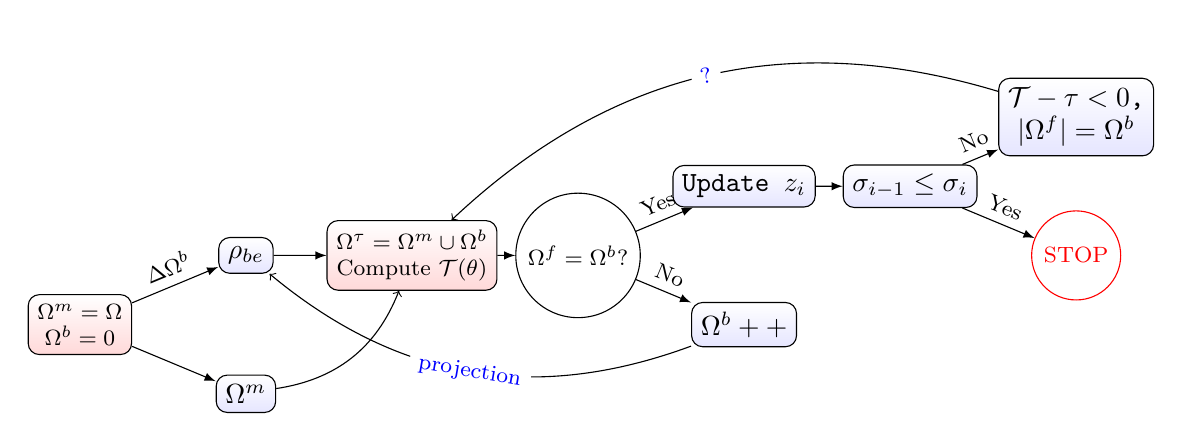
\begin{tikzpicture}
  [
    grow                    = right,
    sibling distance        = 5em,
    level distance          = 6em,
    edge from parent/.style = {draw, -latex},
    every node/.style       = {font=\footnotesize},
    sloped
  ]

  \node [root] (P1){$\Omega^{m}=\Omega$\\$\Omega^{b}=0$}
  child { node [env] (A1) {$\Omega^{m}$}}
  child { node [env] (A) {$\rho_{be}$}
      child { node [root] (B) {$\Omega^{\tau}=\Omega^{m}\cup\Omega^{b}$\\
              Compute $\mathcal{T}(\theta)$}
          child { node [dummy] (C) {$\Omega^{f}=\Omega^{b}$?}
              child{ node [env] (D) {$\Omega^{b}++$}
                  edge from parent node [above] {No}}
              child{ node [env] (E) {Update $z_{i}$}
                  child{ node [env] (F) {$\sigma_{i-1}\leq\sigma_{i}$}
                      child { node [dummy, color=red] (G) {STOP}
                          edge from parent node [above] {Yes}}
                      child { node [env] (H) {$\mathcal{T}-\tau<0$,\\$|\Omega^{f}|=\Omega^{b}$}
                          edge from parent node [above] {No}}}
                  edge from parent node [above] {Yes}}}}
      edge from parent node [above] {$\Delta\Omega^{b}$} };
  \draw[->] (D) edge[bend left] node[midway, color=blue, fill=white]{projection} (A);
  \draw[->] (H) edge[bend right] node[midway, color=blue, fill=white]{?} (B);
  \draw[->] (A1) edge[bend right] (B);
\end{tikzpicture}
\end{document}